\begin{figure}[H]
\centering
\includegraphics[page=6,width=0.48\textwidth]{\FCNCFigures/tthML/showFake/faketau/postfit/NOMINAL/reg1l1tau1b1j_ss_vetobtagwp70_highmet/tau_pt_0.pdf}
%\put(-100, 140){\textbf{(a)}}
%\put(-120, 130){\footnotesize{$l\thad 1j$}}
\includegraphics[page=6,width=0.48\textwidth]{\FCNCFigures/tthML/showFake/faketau/postfit/NOMINAL/reg1l1tau1b2j_ss_vetobtagwp70_highmet/tau_pt_0.pdf}
%\put(-100, 140){\textbf{(b)}}
%\put(-120, 130){\footnotesize{$l\thad 2j$}}

\includegraphics[page=6,width=0.48\textwidth]{\FCNCFigures/tthML/showFake/faketau/postfit/NOMINAL/reg1l1tau1b2j_os_vetobtagwp70_highmet/tau_pt_0.pdf}
%\put(-100, 140){\textbf{(c)}}
%\put(-120, 130){\footnotesize{$STH \tlhad$}}
\includegraphics[page=6,width=0.48\textwidth]{\FCNCFigures/tthML/showFake/faketau/postfit/NOMINAL/reg1l1tau1b3j_os_vetobtagwp70_highmet/tau_pt_0.pdf}
%\put(-100, 140){\textbf{(d)}}
%\put(-120, 130){\footnotesize{$TTH \tlhad$}}

\includegraphics[page=6,width=0.48\textwidth]{\FCNCFigures/tthML/showFake/faketau/postfit/NOMINAL/reg1l2tau1bnj_os/tau_pt_0.pdf}
%\put(-100, 140){\textbf{(e)}}
%\put(-120, 130){\footnotesize{$l\thadhad$}}


\caption{ The data-MC comparison of $\tau$ $\pt$ in the signal regions after the fake tau correction and QCD estimation. }
\label{fig:wjet_pt_postfit}
\end{figure}
